We have seen in \autoref{chapter: RMT} that the j.p.d.f. of eigenvalues of certain random matrices defines a determinantal point processes. We will see that not only that, but eigenvalues can have the same correlation functions as another point process: The so called \textit{Coulomb gas}. These can be though of as a measure on a physical gas of repelling ions restricted to some conductor under a confining potential. With this interpretation one wonders what happens to these gases in the \textit{thermodynamic limit}.  Physically, this is the regime we are used to work with; in thermodynamics we often study macroscopic properties of gases such as \textit{entropy} or \textit{temperature}. When considering a large enough number of particles, fluctuations of these quantities become negligible. Moreover, under the appropriate conditions, to be discussed further in the chapter, these particles are known to converge to a limit equilibrium configuration. In our matrices, these equilibrium configurations will refer to the eigenvalue univariate density function and, as discussed in \autoref{chapter: RMT}, will be expressed by the correlation kernel.

Furthermore, in this chapter we also expand on the usual formulation of minimization of a particle system's energy problems. We begin discussing \textit{equilibrium measures} of eigenvalues - the unique measure that minimizes our functional problem. This minimization lead us to a type of problem can be solved by considering the \textit{Euler-Lagrange}, or \textit{Variational Equations}. We use these results to calculate the equilibrium measures for the ensemble of random matrices we work with in \autoref{chapter: planarensembles}. Finally, we finish this chapter doing some informal calculations that intend to motivate the asymptotic expression we get for the partition function on \autoref{chapter: planarensembles}. This also gives a basis estimate to which we compare the order of approximation obtained in \citeonline{Byun_2023} and explored in \autoref{chapter: planarensembles}. 

We based \autoref{Section: Equilibrium}, on equilibrium measures, on the works of \citeonline{saff2024logarithmic} and \citeonline{deiftorthogonal}. The argument to derive an expression for the free energy in \autoref{Section: Free eenrgy} is presented in \citeonline{Livan_2018}.

\section{Coulomb Gases}
\label{Section: Coulomb Gas}

We start by describing a familiar distribution for physicists: The Boltzmann-Gibbs distribution. This is a probability distribution that represents the probability of a given state for a system of $n$ particles as a function of the system state's \textit{energy} ($\Hf$) and the \textit{temperature} ($1/(\beta n^2)$). Physically, this is the distribution that maximizes the entropy: lower energy states have higher probability of being occupied than states with higher energy.  This distribution is common on thermodynamics by this very reason. Let's introduce a system that has states partitioned accordingly to such distribution. Suppose a set of $n$ particles at positions $\mmany{x}{n} \in \Sigma$, a \textit{conductor} of dimension $d$, or in some configuration $\chi_n = (\mmany{x}{n})$, embedded $\R^{dn}$.
\begin{definicao}
	If $\dd p_n$ is a probability measure on $(\R^d)^n$, we name it \textbf{Coulomb gas} if it has the form of a Boltzmann-Gibbs probability measure, namely if
	\begin{equation}
		\dd p_n(\chi_n) = \frac{\ee^{-\beta n^2 \Hf(\chi_n)}}{\pZ{n, \beta}{Q}} \prod_{i=1}^{n} \dd^d x_i,
		\label{Equation: Coulomb Gas Measure}
	\end{equation}
	where 
	\begin{equation}
		\Hf(\chi_n) = \frac{1}{2n} \sum_{i = 1}^{n} \Q(x_i) + \frac{1}{n^2} \sum_{i < j}^{n} \g(x_i - x_j)	
	\end{equation}
	is usually called the \textbf{Hamiltonian}, or more concretely, the \textbf{configurational energy} of the system. The function $\g \colon \Sigma \rightarrow (-\infty, \infty]$ is the \textit{Coulomb Interacting Kernel}, solution to the Poisson equation and given by 
	$
	\g(x) = - \ln(|x|)
	$ for $d = 1, 2$.
	The function $\Q \colon \R^d \cong \Sigma \rightarrow \R$ is the external potential and $\pZ{n,\beta}{Q}$ is the \textbf{partition function}, or normalization function, given by
	\begin{equation}
		\pZ{n,\beta}{Q} = \int_{\R^{dn}}  \ee^{-\beta n^2 \Hf(\chi_n)}  \prod_{i=1}^{n} \dd^d x_i.
	\end{equation}
\end{definicao}
The measure $\dd p_n$ models an Coulomb-interacting gas of charged indistinguishable particles under some external field $\Q$. We wish $\dd p_n$ to be a probability measure,  then one must ensure that $\Q$ is such that the normalizing constant $\pZ{n,\beta}{Q}$ is finite for all $n$. This is all to say that the potential should be confining: As the number of particles increases, it must counter the repulsion effect and keep limited the region where particles move around. Recall the expression for the orthogonal polynomial ensembles in \autoref{Definition: polynomial ensemble}. As we are dealing with point processes on the plane, we take the gas to be in a two dimensional conductor ($d = 2$) and $\beta = 2$. Rearranging the terms in \eqref{Equation: Coulomb Gas Measure} we get
\begin{equation}
	\dd p_n(\mmany{z}{n}) = \frac{1}{\pZ{n}{Q}}\prod_ {i < j}^n |z_i - z_j|^2 \prod_{j=i}^{n} \ee^{- n \Q(z_i)} \dd^2 z_i.
\end{equation}
The similarity to \autoref{Definition: polynomial ensemble} indicates that eigenvalues from invariant ensembles share some statistics with Coulomb gases. This opens the way for interpretations of the distribution of eigenvalues but also to computations using simulation methods for particle dynamics, see \autoref{Exemplo: TCC complex potential}. This also motives why most often the weight functions used for invariant ensembles will have the form, for $Q$ polynomial,
\begin{equation} \label{Equation: weight funciton form}
	\wf(x) = \ee^{-n \Q(x)}.
\end{equation}
This directly relates to the weight function in \autoref{Definition: polynomial ensemble} and gives a way to trap particles in a limited set - giving smaller probabilities for configurations with more diffused particles.

\begin{exemplo} \label{Exemplo: TCC complex potential}
	As explored in \citeonline{Chafal}, a few classical algorithms of simulation are very successful in replicating the measures for Coulomb gas systems. Equivalently, if one is interested in sampling eigenvalues for our invariant ensembles, one can sample from its configuration equilibrium $\p_Q(\lambda)$ with respect to some potential $Q$ using simulation of the particles. Consider for example the non-trivial case explored in \citeonline{balogh2016orthogonal}, where, taken $d = 2$ and $n = 2$ we will have $W(x) = g(x) = \log{|x|}$ and impose the potential
	\begin{equation}
		Q(z)=|z|^{2a} - \re{t z^a}.
		\label{Equation: Complex Potential}
	\end{equation}
	This potential has disjoint intervals for some combinations of the parameters $t$ and $a$ - it presents a transition in $t_c \approx \sqrt{(1/a)}$. Analytically, it was just recently solved. However we can easily sample from this measure using particle simulations, as shown below. Data was taken from \citeonline{TCCJoaoPimenta}.
	\begin{figure}[H]
		\pgfplotsset{width=5cm,compat=1.9}
		\begin{subfigure}{0.2\textwidth}
			\centering
			\begin{tikzpicture}
				\begin{axis}[axis line style={opacity=0}, ticks=none,
					xmin=-1.5, xmax=1.5,
					ymin=-1.5, ymax=1.5,
					xticklabel=\empty,
					yticklabel=\empty,
					xlabel={t = 0},
					ylabel={a = 2},
					xticklabel pos=top,
					scatter/classes={%
						a={ mark size=0.5pt}}
					]
					\addplot[skip coords between index={50}{500}, opacity=1, scatter, mark=x, black, only marks] table [col sep=comma] {./plotdata/Symmetric/5lines/a2t0.csv};
					\addplot[opacity=0.05, scatter, mark=*,draw opacity=0,black, only marks] table [col sep=comma] {./plotdata/Symmetric/5lines/a2t0.csv};
				\end{axis}
			\end{tikzpicture}
		\end{subfigure} \hspace{1cm}
		\begin{subfigure}{0.2\textwidth}
			\centering
			\begin{tikzpicture}
				\begin{axis}[axis line style={opacity=0}, ticks=none,
					xmin=-1.5, xmax=1.5,
					ymin=-1.5, ymax=1.5,
					xlabel={t = 0.5},
					xticklabel pos=top,
					xticklabel=\empty,
					yticklabel=\empty,
					scatter/classes={%
						a={ mark size=0.5pt}}
					]
					\addplot[skip coords between index={50}{500}, opacity=1, scatter, mark=x, black, only marks] table [col sep=comma] {./plotdata/Symmetric/5lines/a2t05.csv};
					\addplot[opacity=0.05, scatter, mark=*,draw opacity=0,black, only marks] table [col sep=comma] {./plotdata/Symmetric/5lines/a2t05.csv};
				\end{axis}
			\end{tikzpicture}
		\end{subfigure} \hfill
		\begin{subfigure}{0.2\textwidth}
			\centering
			\begin{tikzpicture}
				\begin{axis}[axis line style={opacity=0}, ticks=none,
					xmin=-1.5, xmax=1.5,
					ymin=-1.5, ymax=1.5,
					xlabel={t = 1},
					xticklabel pos=top,
					xticklabel=\empty,
					yticklabel=\empty,
					scatter/classes={%
						a={ mark size=0.5pt}}
					]
					\addplot[skip coords between index={50}{500}, opacity=1, scatter, mark=x, black, only marks] table [col sep=comma] {./plotdata/Symmetric/5lines/a2t1.csv};
					\addplot[opacity=0.05, scatter, mark=*,draw opacity=0,black, only marks] table [col sep=comma] {./plotdata/Symmetric/5lines/a2t1.csv};
				\end{axis}
			\end{tikzpicture}
		\end{subfigure} \hfill
		\begin{subfigure}{0.2\textwidth}
			\centering
			\begin{tikzpicture}
				\begin{axis}[axis line style={opacity=0}, ticks=none,
					xmin=-1.5, xmax=1.5,
					ymin=-1.5, ymax=1.5,
					xlabel={t = 2},
					xticklabel=\empty,
					yticklabel=\empty,
					xticklabel pos=top,
					scatter/classes={%
						a={ mark size=0.5pt}}
					]
					\addplot[skip coords between index={50}{500}, opacity=1, scatter, mark=x, black, only marks] table [col sep=comma] {./plotdata/Symmetric/5lines/a2t2.csv};
					\addplot[opacity=0.05, scatter, mark=*,draw opacity=0,black, only marks] table [col sep=comma] {./plotdata/Symmetric/5lines/a2t2.csv};
				\end{axis}
			\end{tikzpicture}
		\end{subfigure} \hfill
	\end{figure}
	\begin{figure}[H]
		\pgfplotsset{width=5cm,compat=1.9}
		\begin{subfigure}{0.2\textwidth}
			\centering
			\begin{tikzpicture}
				\begin{axis}[axis line style={opacity=0}, ticks=none,
					xmin=-1.5, xmax=1.5,
					ymin=-1.5, ymax=1.5,
					xticklabel=\empty,
					yticklabel=\empty,
					ylabel={a = 3},
					scatter/classes={%
						a={ mark size=0.5pt}}
					]
					\addplot[skip coords between index={50}{500}, opacity=1, scatter, mark=x, black, only marks] table [col sep=comma] {./plotdata/Symmetric/5lines/a3t0.csv};
					\addplot[opacity=0.05, scatter, mark=*,draw opacity=0,black, only marks] table [col sep=comma] {./plotdata/Symmetric/5lines/a3t0.csv};
				\end{axis}
			\end{tikzpicture}
		\end{subfigure} \hspace{1cm}
		\begin{subfigure}{0.2\textwidth}
			\centering
			\begin{tikzpicture}
				\begin{axis}[axis line style={opacity=0}, ticks=none,
					xmin=-1.5, xmax=1.5,
					ymin=-1.5, ymax=1.5,
					xticklabel=\empty,
					yticklabel=\empty,
					scatter/classes={%
						a={ mark size=0.5pt}}
					]
					\addplot[skip coords between index={50}{500}, opacity=1, scatter, mark=x, black, only marks] table [col sep=comma] {./plotdata/Symmetric/5lines/a3t05.csv};
					\addplot[opacity=0.05, scatter, mark=*,draw opacity=0,black, only marks] table [col sep=comma] {./plotdata/Symmetric/5lines/a3t05.csv};
				\end{axis}
			\end{tikzpicture}
		\end{subfigure} \hfill
		\begin{subfigure}{0.2\textwidth}
			\centering
			\begin{tikzpicture}
				\begin{axis}[axis line style={opacity=0}, ticks=none,
					xmin=-1.5, xmax=1.5,
					ymin=-1.5, ymax=1.5,
					xticklabel=\empty,
					yticklabel=\empty,
					scatter/classes={%
						a={ mark size=0.5pt}}
					]
					\addplot[skip coords between index={50}{500}, opacity=1, scatter, mark=x, black, only marks] table [col sep=comma] {./plotdata/Symmetric/5lines/a3t1.csv};
					\addplot[opacity=0.05, scatter, mark=*,draw opacity=0,black, only marks] table [col sep=comma] {./plotdata/Symmetric/5lines/a3t1.csv};
				\end{axis}
			\end{tikzpicture}
		\end{subfigure} \hfill
		\begin{subfigure}{0.2\textwidth}
			\centering
			\begin{tikzpicture}
				\begin{axis}[axis line style={opacity=0}, ticks=none,
					xmin=-1.5, xmax=1.5,
					ymin=-1.5, ymax=1.5,
					xticklabel=\empty,
					yticklabel=\empty,
					scatter/classes={%
						a={ mark size=0.5pt}}
					]
					\addplot[skip coords between index={50}{500}, opacity=1, scatter, mark=x, black, only marks] table [col sep=comma] {./plotdata/Symmetric/5lines/a3t2.csv};
					\addplot[opacity=0.05, scatter, mark=*,draw opacity=0,black, only marks] table [col sep=comma] {./plotdata/Symmetric/5lines/a3t2.csv};
				\end{axis}
			\end{tikzpicture}
		\end{subfigure} \hfill
	\end{figure}
	\begin{figure}[H]
		\pgfplotsset{width=5cm,compat=1.9}
		\begin{subfigure}{0.2\textwidth}
			\centering
			\begin{tikzpicture}
				\begin{axis}[axis line style={opacity=0}, ticks=none,
					xmin=-1.5, xmax=1.5,
					ymin=-1.5, ymax=1.5,
					xticklabel=\empty,
					yticklabel=\empty,
					ylabel={a = 5},
					scatter/classes={%
						a={ mark size=0.5pt}}
					]
					\addplot[skip coords between index={50}{500}, opacity=1, scatter, mark=x, black, only marks] table [col sep=comma] {./plotdata/Symmetric/5lines/a5t0.csv};
					\addplot[opacity=0.05, scatter, mark=*,draw opacity=0,black, only marks] table [col sep=comma] {./plotdata/Symmetric/5lines/a5t0.csv};
				\end{axis}
			\end{tikzpicture}
		\end{subfigure} \hspace{1cm}
		\begin{subfigure}{0.2\textwidth}
			\centering
			\begin{tikzpicture}
				\begin{axis}[axis line style={opacity=0}, ticks=none,
					xmin=-1.5, xmax=1.5,
					ymin=-1.5, ymax=1.5,
					xticklabel=\empty,
					yticklabel=\empty,
					scatter/classes={%
						a={ mark size=0.5pt}}
					]
					\addplot[skip coords between index={50}{500}, opacity=1, scatter, mark=x, black, only marks] table [col sep=comma] {./plotdata/Symmetric/5lines/a5t05.csv};
					\addplot[opacity=0.05, scatter, mark=*,draw opacity=0,black, only marks] table [col sep=comma] {./plotdata/Symmetric/5lines/a5t05.csv};
				\end{axis}
			\end{tikzpicture}
		\end{subfigure} \hfill
		\begin{subfigure}{0.2\textwidth}
			\centering
			\begin{tikzpicture}
				\begin{axis}[axis line style={opacity=0}, ticks=none,
					xmin=-1.5, xmax=1.5,
					ymin=-1.5, ymax=1.5,
					xticklabel=\empty,
					yticklabel=\empty,
					scatter/classes={%
						a={ mark size=0.5pt}}
					]
					\addplot[skip coords between index={50}{500}, opacity=1, scatter, mark=x, black, only marks] table [col sep=comma] {./plotdata/Symmetric/5lines/a5t1.csv};
					\addplot[opacity=0.05, scatter, mark=*,draw opacity=0,black, only marks] table [col sep=comma] {./plotdata/Symmetric/5lines/a5t1.csv};
				\end{axis}
			\end{tikzpicture}
		\end{subfigure} \hfill
		\begin{subfigure}{0.2\textwidth}
			\centering
			\begin{tikzpicture}
				\begin{axis}[axis line style={opacity=0}, ticks=none,
					xmin=-1.5, xmax=1.5,
					ymin=-1.5, ymax=1.5,
					xticklabel=\empty,
					yticklabel=\empty,
					scatter/classes={%
						a={ mark size=0.5pt}}
					]
					\addplot[skip coords between index={50}{500}, opacity=1, scatter, mark=x, black, only marks] table [col sep=comma] {./plotdata/Symmetric/5lines/a5t2.csv};
					\addplot[opacity=0.05, scatter, mark=*,draw opacity=0,black, only marks] table [col sep=comma] {./plotdata/Symmetric/5lines/a5t2.csv};
				\end{axis}
			\end{tikzpicture}
		\end{subfigure} \hfill
		\caption{Shown in the shadow is the mean configurations - in some an approximation of the limit distribution of points, and in the scatter is a random $n = 50$ sample from the distribution. We show configurations for combinations of the parameters $t = 0, 0.5, 1, 2$ from left ro right and $a = 2, 3, 5$ from top to bottom.}
	\end{figure}
\end{exemplo}

\section{Equilibrium Measures}
\label{Section: Equilibrium}

The description of the eigenvalues as a \textit{Coulomb gas} discussed in \autoref{Section: Coulomb Gas} and as a \textit{point process} in \autoref{Section: RMT} raises some ways to think of this system of particles. Especially, when dealing with the large $n$ limit, the physical interpretation of this system as a interacting gas lead us to the idea of minimizing the energy of the system. In such minimization the particles should find themselves in what we call an equilibrium configuration  $\chi_n = \{\mmany{z}{n}\}$. In the large $n$ limit, under some mild conditions to be discussed, the counting measure defined with respect to this configuration converges to a continuous measure with compact support. This limit object is what we call an \textit{equilibrium measure}. To clarify the point, suppose we are dealing with the j.p.d.f.
\begin{equation} \label{Equation: Equilibrium gas}
	p_n(\chi_n) = \frac{\ee^{- n^2 \Hf(\chi_n)}}{\pZ{n}{Q}}, \quad \Hf(\chi_n) = \frac{1}{n} \sum_{i = 1}^{n} Q(z_i) + \frac{1}{n^2} \sum_{i \neq j}^{n} \ln{\frac{1}{|z_i - z_j|}}. 
\end{equation}
For any $n$-configuration ${\chi_n} = \{\mmany{z}{n}\}$, let $\mu_{\chi_n}$ be the normalized counting measure on $\C$,
\begin{equation}
	\mu_{\chi_n} = \frac{1}{n} \sum_{i=1}^{n} \delta_{z_i}, \quad \text{such that} \quad \int_{\C} \dd \mu_{\chi_n} = 1.
 \end{equation} 
 Then
\begin{equation}
	\frac{1}{n^2} \sum_{i \neq j} \ln{|z_i - z_j|^{-1}} + \frac{1}{n} \sum_{i=1}^n \Q(z_i) 
\end{equation}
may be written in the form 
\begin{equation}
	\int \int_{t \neq s} \ln |t - s|^{-1} \dd \mu_{\chi_n}(t) \dd \mu_{\chi_n}(s) + \int \Q(s) \dd  \mu_{\chi_n} (s).
\end{equation}
This lead us, think of the convergence of $\mu_{\chi_n} \rightarrow \mu$, to the energy minimization problem 
\begin{align}
	E^{(\Q)} & = \inf_{\mu \in \M^1(\C)} \left[ \int \int_{t \neq s} \ln |t - s|^{-1} \dd \mu(t) \dd \mu(s) + \int \Q(s) \dd  \mu(s) \right] \\ & = \inf_{\mu \in \M^1(\C)} \left[ I_\Q(\mu) \right]
\end{align}
where
\begin{equation}
	\M^1(\C) = \left\{ \mu \in \text{Borel measures on} \ \C \ \bigg| \int \dd \mu = 1 \right\}.
\end{equation}

The quantity $E^{(Q)}$ is the \textit{equilibrium energy} of the system and $I_Q(\mu_{\chi_n})$ is the \textit{energy integral}. For $\mu_Q$, the equilibrium measure for the minimization problem above, to be compact, $\Q$ the confining potential, must essentially be finite in such set and increase sufficiently fast around infinity. However, to analyze this case, we first consider the simplified version without an external potential. Let $\Sigma \subseteq \C$ be a compact subset of the complex plane and $\M(\Sigma)$ be the collection of all positive Borel measure of compact support in $\Sigma$. Let $\mu \in \M(\Sigma)$ be such a measure in the complex plane $\C$.
\begin{definicao}
	 The associated \textbf{logarithmic potential} of a finite measure $\mu$ is defined by 
	\begin{equation}
		U^{\mu}(z) \deff \int \ln \frac{1}{|z - t|} \dd \mu(t).
	\end{equation}
	Also, $I(\mu)$, called the \textbf{logarithmic energy} of $\mu \in \M(\Sigma)$ is defined by
	\begin{equation}
		I(\mu) \deff \int \int_{z \neq t} \ln \frac{1}{|z-t|} \dd \mu(z) \dd \mu (t),
	\end{equation}
	the \textbf{energy} $V$ of $\Sigma$ is
	\begin{equation}
		V \deff \inf\{ I(\mu) | \mu \in \M(\Sigma)\}.
	\end{equation}
	If $V$ is finite, then the measure $\mu^V_\Sigma$ which minimizes the energy, is called the \textbf{equilibrium measure}.
\end{definicao}

This logarithmic potential can be easily interpreted if one reconsiders the Coulomb gas analogy discussed in \autoref{Section: Coulomb Gas}. Note that the interaction between two particles of gas we considered is logarithmic. Then, taking the empirical counting measure $\mu_{\chi_n}$,
\begin{equation}
	U^{	\mu_{\chi_n}}(z) = \int \ln \frac{1}{|z - t|} \dd \mu_{\chi_n}(t) = \sum_{i=1}^n \ln \frac{1}{|z  - \lambda_i|}.
\end{equation}
This is precisely the potential created by the particles interactions on the point $z$. There are a few useful properties one can extract about this quantity. A similar argument can also be made to justify the logarithmic energy. 

\begin{proposicao} \cite{saff2024logarithmic}
	Let $\mu$ be a finite positive Borel measure of compact support on the complex plane $\C$. Then the logarithmic potential is super-harmonic on the whole plane, that is, it has the following properties.
	\begin{enumerate}
		\item $U^{\mu}(z) > -\infty$ for all $z$,
		\item $U^{\mu}$ is lower semi-continuous,
		\item $U^{\mu}(z) \geq \frac{1}{2\pi} \int_{-\pi}^{\pi} U^{\mu}(z + r \ee^{\ii \theta}) \dd \theta$ for all $z$ and all $r \geq 0$. 
	\end{enumerate}
\end{proposicao}
\begin{proof}
	Firstly, property $(1)$ follows directly by $(2)$, since a lower semi-continuous function is everywhere $> -\infty$ and $\mu$ has compact support. Property $(2)$ is proven noticing that
	\begin{equation}
		U^\mu(z) = \lim_{M \rightarrow \infty} \int \min\left( M, \ln \frac{1}{|z - t|} \right) \dd \mu (t).
	\end{equation}
	The functions on the right-hand side are continuous and increasing with $M$, and limit of an increasing sequence of functions must be lower semi-continuous. To prove $(3)$, note that the kernel $\ln(1/|z-t|)$ is super-harmonic in $\C$ for each $t$. If some $F$ is analytic in a domain $D$ and $\rho > 0$, then $|F(z)|^\rho$ is sub-harmonic in $D$; furthermore, $\ln |F(z)|$ is sub-harmonic in $D$ provided $F$ is not identically zero. Thus, 
	\begin{equation}
		\frac{1}{2\pi} \int_{-\pi}^{\pi} \ln{\frac{1}{|z - r\ee^{\ii \theta} - t|}} \dd \theta \leq \ln \frac{1}{|z-t|}, \quad z, t \in \C.
	\end{equation}
	Using the Fubini-Toneli theorem and the inequality above
	\begin{align}
		\frac{1}{2\pi} \int_{-\pi}^{\pi} U^\mu (z + r \ee^{\ii \theta}) \dd \theta & = \int \frac{1}{2\pi} \int_{-\pi}^{\pi} \ln{\frac{1}{|z - r\ee^{\ii \theta} - t|}} \dd \theta \dd \mu(t), \\
		& \leq \int \ln \frac{1}{|z-t|} \dd \mu(t) = U^\mu (z).
	\end{align}
\end{proof}

For technical reasons we also state \autoref{Lema: positive kernel} regarding the logarithmic energy that will become useful in a later result but to which we do not provide a proof.

\begin{lema} 	\label{Lema: positive kernel}
	\cite{saff2024logarithmic}
	Let $\mu = \mu_1 - \mu_2$ be a signed Borel measure with compact support	and total mass $\mu(\C) = 0$. Suppose further that each of the positive measures $\mu_1$ and $\mu_2$ has finite logarithmic energy. Then the logarithmic energy of $\mu$
	\begin{equation}
		I(\mu) = \int \int \ln \frac{1}{|z-t|} \dd \mu(z) \dd \mu (t),
	\end{equation}
	is non-negative and it is zero if and only if $\mu \equiv 0$.
\end{lema}

Suppose that there is a unique measure $ \mu^V_\Sigma \in \M(\Sigma)$ for which the minimum energy $V = \inf\{ I(\mu) | \mu \in \M(\Sigma)\}$ is finite and reachable. Such a measure $\mu^V_\Sigma$ is called the \textit{equilibrium distribution} or \textit{equilibrium measure} of the compact set $\Sigma$. These concepts have a natural electrostatic interpretation. Suppose $\Sigma$ is a conductor and charged particles are placed on it. If the force between the particles is proportional to the reciprocal of their distance and $Q$ is some external field to which they interact to, then $\mu^V_\Sigma$ is the configuration which minimizes the energy, or maximizes the entropy, of the system. This measure gives the distribution to which this particles are in equilibrium. 

We should at this point reintroduce the external potential $Q$. Most often than not, an external force will change the minimum energy state and equilibrium configurations. Particles tend to accumulate at the minimum of such potential. The reason why the distribution will not be a single point in space is that the logarithmic energy, from the interactions, explodes when particles are close by. For this case, a weighted version of the problem was developed. The main difference now is that $\Sigma$ is not required to be compact; we only impose that there is no positive mass around infinity. There is a natural way to enforce these conditions. Let $\Sigma \subset \C$ be a closed set and $\wf : \Sigma \rightarrow [0, \infty)$. This function $\wf$ is called a \textit{weight function} on $\Sigma$. Certain weight functions make it so that there is no positive mass around infinity; we call such function \textit{admissible}.

\begin{definicao}	\label{Definition: Weight Admissibility}
	Define also the \textit{logarithmic capacity} to be	$\cpct{(\Sigma)} = \ee^{-V}$ with $V = \inf\{ I(\mu) | \mu \in \M(\Sigma)\}$. A weight function $\wf = \ee^{-nQ(z)}$ is said to be \textbf{admissible} is it satisfies the following three conditions
	\begin{enumerate}
		\item Q is upper semi-continuous;
		\item $\Sigma_0 \deff \{ z \in \Sigma | Q > -\infty \}$ has positive capacity;
		\item if $\Sigma$ is unbounded, then $\liminf_{|z| \rightarrow \infty } \frac{Q(z)}{2 \ln{(|z|)}} > 1$ as $|z| \rightarrow \infty$, $z \in \Sigma$.
	\end{enumerate} 
\end{definicao}

Let $\M(\Sigma)$ be the collection of all positive unit Borel measures $\mu$ with support in $\Sigma$. Our definition for the weighted energy integral now reads
\begin{equation}
	I_Q(\mu) = \int U^\mu(s)  \dd \mu(s) + \int \Q(s) \dd  \mu(s),
\end{equation}
for $\mu \in \M(\Sigma)$ and is recovered if both integrals exist and are finite. Note that this is to say that
\begin{align}
	I_Q(\mu) & = \int U^\mu(s)  \dd \mu(s) + \int \Q(s) \dd  \mu(s), \\
	& = \int \int_{s \neq t} \ln \frac{1}{|s-t|} \dd \mu(s) \dd \mu (t) + \frac{1}{2} \left[ \int \Q(s) \dd  \mu(s) + \int \Q(t) \dd  \mu(t)  \right], \\
	& =   \int \int_{s \neq t} \left( \ln \frac{1}{|s-t|} + \frac{\Q(t)}{2} + \frac{\Q(s)}{2} \right) \dd \mu(s) \dd \mu (t), \\
	& = \int \int_{s \neq t} \kappa^Q(s,t) \dd \mu(s) \dd \mu (t)
\end{align}
converges. Denote
\begin{equation}
	\phi^Q(x) = Q(x) - \ln(x^2 + 1)
\end{equation}
and note that
\begin{equation}
	\ln |t - s|^{-1} \geq - \frac{1}{2} \ln(1+t^2) - \frac{1}{2} \ln(1+s^2).
\end{equation}
Therefore
\begin{equation}
	\kappa^Q(s,t) \geq \frac{1}{2}\phi^Q(t) + \frac{1}{2}\phi^Q(s)\geq c_Q > -\infty
\end{equation}
since $\lim_{|x|\rightarrow \infty}\phi^Q(x) = \infty$ and $\phi^Q(x) \geq c_Q > -\infty$. Thus, $I_Q \geq c_Q > -\infty$ for every $\mu \in \M^1(\C)$. Remember that we are dealing with weight functions of the form
$
	\wf(z) = \ee^{-nQ(z)}
$
for $z \in \C$ and we want $Q$ to be such that the weighted logarithmic energy is finite - the weight is admissible. Then, by the definition, $Q : \Sigma \rightarrow (\infty, \infty]$ must be lower semi-continuous. To avoid degeneracy, we imposed that $Q < \infty$ in some set of positive capacity. Furthermore, we must have that $\liminf_{|z| \rightarrow \infty } \frac{Q(z)}{2 \ln{(|z|)}} > 1$ such that the potential energy grows faster than the interaction logarithmic energy. Remember that this is similar to the condition imposed on the orthogonal polynomial ensembles in \autoref{Definition: polynomial ensemble}. On the next section we move on to the matter of determining the \textit{equilibrium measure} $\mu_Q$ for a given external field $\Q$.

\begin{teorema} \cite{saff2024logarithmic}
	Let $\wf$ be an admissible weight function on the closed set $\Sigma$ and let 
	\begin{equation}
		V_\wf \deff \inf \{I_\wf(\mu) | \mu \in \mathcal{M}(\Sigma)\}.
	\end{equation}
	Then, $V_\wf$ is finite and there exists a unique element $\mu_\wf \in$ such that $I_\wf(\mu_\wf) = V_\wf$.
\end{teorema}
On the next section we move on to the matter of determining the \textit{equilibrium measure} $\mu_Q$ for a given external field $\Q$.

\begin{exemplo}
	Take the Coulomb gas measure described in \autoref{Section: Coulomb Gas}, and restrict the conductor $\Sigma$ to be the real line under the external potential
	\begin{equation}
		Q(x) = t x^{2m}.
	\end{equation}
	By finding configurations that minimizes the Hamiltonian, one also finds the more likely configurations. These configurations, when $n \rightarrow \infty$ converges to a measure $\mu_Q$ that minimizes the logarithmic energy. It can be shown that this measure is given by
	\begin{equation}
		\supp \mu_Q(x) = [-a, a], \quad \mu_Q(x) = \frac{mt}{\pi} \sqrt{a^2 - x^2} h(x),
		\label{Equation: Monic external potential}
	\end{equation}
	where
	\begin{equation}
		a \deff \left( mt \prod_{l=1}^{m} \frac{2l-1}{2l}\right)  \quad \text{and} \quad h(x) \deff x^{2m-2} + \sum_{j=1}^{m-1} x^{2m-2-2j} a^{2j} \prod_{l=1}^{j} \frac{2l-1}{2l}.
	\end{equation}	
	See \citeonline{deiftorthogonal} for details. Note that this simplifies to the Gaussian case if $Q(x) = x^2/2$ ($t, m=1$). In such case we already shown that the equilibrium measure is defined by the Semicircle distribution
	\begin{equation}
		\supp{\mu_Q(x)} = [-\sqrt{2}, \sqrt{2}], \ \ \ \mu_Q(x) = \frac{1}{\pi} \sqrt{2 - x^2}.
		\label{Equation: Gaussian external potential}
	\end{equation}
		\begin{figure}[H]
		\pgfplotsset{width=4.9cm,compat=1.9}
		\begin{subfigure}{0.22\textwidth}
			\centering
			\begin{tikzpicture}
				\begin{axis}[
					xmin=-1.6, xmax=1.6,
					ymin=0, ymax=0.85,
					title= {$m=1$}
					]
					\addplot [ thin, opacity=0.5,
					hist={density, bins=20}
					] table [y index=0] {./plotdata/Monic/Monict0a0.csv};
					\addplot[solid, black, thick] table [col sep=comma] {./plotdata/Monic/MonicFunct0a0.csv};
				\end{axis}
			\end{tikzpicture}
		\end{subfigure} \hspace{0.75cm}
		\begin{subfigure}{0.22\textwidth}
			\centering
			\begin{tikzpicture}
				\begin{axis}[
					xmin=-1.6, xmax=1.6,
					ymin=0, ymax=0.85,
					title= {$m=2$},
					yticklabel=\empty
					]
					\addplot [ thin, opacity=0.5,
					hist={density, bins=20}
					] table [y index=0] {./plotdata/Monic/Monict0a1.csv};
					\addplot[solid, black, thick] table [col sep=comma] {./plotdata/Monic/MonicFunct0a1.csv};
				\end{axis}
			\end{tikzpicture}
		\end{subfigure} \hfill
		\begin{subfigure}{0.22\textwidth}
			\centering
			\begin{tikzpicture}
				\begin{axis}[
					xmin=-1.6, xmax=1.6,
					ymin=0, ymax=0.85,
					title= {$m=3$},
					yticklabel=\empty
					]
					\addplot [ thin, opacity=0.5,
					hist={density, bins=20}
					] table [y index=0] {./plotdata/Monic/Monict0a2.csv};
					\addplot[solid, black, thick] table [col sep=comma] {./plotdata/Monic/MonicFunct0a2.csv};
				\end{axis}
			\end{tikzpicture}
		\end{subfigure} \hfill
		\begin{subfigure}{0.22\textwidth}
			\centering
			\begin{tikzpicture}
				\begin{axis}[
					xmin=-1.6, xmax=1.6,
					ymin=0, ymax=0.85,
					title= {$m=5$},
					yticklabel=\empty
					]
					\addplot [ thin, opacity=0.5,
					hist={density, bins=20}
					] table [y index=0] {./plotdata/Monic/Monict0a3.csv};
					\addplot[solid, black, thick] table [col sep=comma] {./plotdata/Monic/MonicFunct0a3.csv};
				\end{axis}
			\end{tikzpicture}
		\end{subfigure} \hfill
		\caption{Four conditions for the Monic potential, the equilibrium measure is expressed by the line plot. For all cases we used $t=1$ and set $m=1,2,3,5$ from left to right. The bin-plot is the result of the simulation of the equivalent Coulomb Gas taken from \citeonline{TCCJoaoPimenta}. }
	\end{figure}
\end{exemplo}

\subsection{Euler-Lagrange}

Associated with the variational problem introduced in \autoref{Section: Equilibrium} defined by
\begin{align} \label{Equation: minimization problem}
	E^{\wf} & = \inf_{\mu \in \M^1} I_Q (\mu), \\
	& =   \inf_{\mu \in \M^1} \left[ \int \int \ln |t - s|^{-1} \dd \mu(t) \dd \mu(s) + \int \Q(s) \dd  \mu(s) \right], \\
	&  = I_Q (\mu_Q),
\end{align}
one defines the so-called \textit{Euler-Lagrange} type variational equations. They are important as they provide a tool to solve these equations for the equilibrium measure $\mu_Q$.

\begin{teorema} \label{Theorem: EL} (Variational Equations)
	The equilibrium measure $\mu_Q$ for the given variational problem in \eqref{Equation: minimization problem}, where $\Sigma = \C$ satisfies the following conditions. There exists a real constant $l$ such that 
	\begin{enumerate}
		\item
		\begin{equation}
			\int \left[ 2 \int \ln{|x-y|^{-1}} \dd \mu_Q(y) + \Q(x) \right] \dd \tilde{\mu}(x) \geq l
		\end{equation}
		for all $\tilde{\mu} \in \M^1(\C)$ of compact support with $I_Q(\tilde{\mu}) < \infty$.
		\item
		\begin{equation}
			2 \int \ln{|x-y|^{-1}} \dd \mu_Q(y) + \Q(x) = l
		\end{equation}
		for $\mu_Q$-almost everywhere.
	\end{enumerate}
	Conversely, if $\mu \in \M^1(\C)$ has compact support, satisfies conditions $(1)$ and $(2)$ above, and $I_Q(\mu) < \infty$, then $\mu = \mu_Q$.
\end{teorema}

\begin{proof}
	The argument of the proof is based on  \cite{deiftorthogonal}. 
	
	($\implies$) We recall that $\mu_Q$ has compact support and $I_Q(\mu_Q) = E^\wf < \infty$. Suppose $\mu^* \in \M^1(\C)$ has compact support and $I_Q(\mu^*) < \infty$. Then, defining a convex combination
	\begin{equation}
		\mu_t = t \mu^* + (1-t) \mu_Q = \mu_Q + t (\mu^* - \mu_Q) \in \M^1(\C), \quad 0 \leq t \leq 1,
	\end{equation}
	we have
	\begin{multline}
		I_Q(\mu_t) = \int \int \ln |t - s|^{-1} \dd \mu_Q(t) \dd \mu_Q(s) + \int \Q(s) \dd  \mu_Q(s) \\
		+ 2t \int \int \ln |t - s|^{-1} \dd \mu_Q(t) \dd (\mu^* - \mu_Q)(s) \\
		+ t  \int \Q(s) \dd  (\mu^* - \mu_Q) (s) \\
		+ t^2 \int \int \ln |t - s|^{-1} \dd (\mu^* - \mu_Q) \dd (\mu^* - \mu_Q)(s).
	\end{multline}
	Each term on the right is finite since $\mu_Q, \mu^*$ have compact support and $I_Q (\mu_Q), I_Q(\mu^*) < \infty$. As $I_Q(\mu_t) \geq I_Q (\mu_Q)$ for $0 \leq t \leq 1$ by assumption of minimality and \autoref{Lema: positive kernel}, is is necessary that
	\begin{equation}
		\int \left[ 2 \int \ln{|x-y|^{-1}} \dd \mu_Q(y) + \Q(x) \right] \dd (\mu^* - \mu_Q)(x) \geq 0
		\label{Equation: Proof Euler >0}
	\end{equation}   
	and therefore
	\begin{equation}
		\int \left[ 2 \int \ln{|x-y|^{-1}} \dd \mu_Q(y) + \Q(x) \right] \dd \mu^*(x) \geq l
		\label{Equation: Proof Euler >l}
	\end{equation}
	where
	\begin{equation}
		\int \left[ 2 \int \ln{|x-y|^{-1}} \dd \mu_Q(y) + \Q(x) \right] \dd \mu_Q(x) \deff l
	\end{equation}
	proving the first assertion in $(1)$. Now, let
	\begin{equation}
		B = \left\{ x \ \bigg| \ 2 \int \ln{|x-y|^{-1}} \dd \mu_Q(y) + \Q(x) < l \right\}.
	\end{equation}
	Then, $B$ must be a bounded set of $\C$. Suppose $\mu^*(B) > 0$ and set
	\begin{equation}
		\mu^*_B = \frac{\chi_B}{\mu^*(B)} \mu^*
	\end{equation}
	where $\chi_B$ is the characteristic function of the set $B$. Then $\mu^*_B \in \M^1(\C)$ has compact support and $I_Q(\mu^*) < \infty$. inserting $\dd \mu^*_B$ in \eqref{Equation: Proof Euler >l}, we find
	\begin{equation}
		l \leq \int \left[ 2 \int \ln{|x-y|^{-1}} \dd \mu_Q(y) + \Q(x) \right] \dd \mu^*_B(x) < l
	\end{equation}
	a contradiction. Therefore, 
	\begin{equation}
		\mu^*(B) = \mu^*\left( \left\{ x \ \bigg| \ 2 \int \ln{|x-y|^{-1}} \dd \mu_Q(y) + \Q(x) < l \right\} \right) = 0
	\end{equation}
	for all measures $\mu^* \in \M^1(\C)$ with support compact and $I_Q(\mu^*) < \infty$. in particular, it is true for $\mu^* = \mu_Q$. Since,
	\begin{align}
		0 & =  \int \left[ 2 \int \ln{|x-y|^{-1}} \dd \mu_Q(y) + \Q(x) - l \right] \dd \mu_Q(x) \\
		& = \int_{\C - B} \left[ 2 \int \ln{|x-y|^{-1}} \dd \mu_Q(y) + \Q(x) - l \right] \dd \mu_Q(x)
	\end{align}
	and $(2)$ follows.
	
	($\impliedby$) If, now, $\mu \in \M^1$ satisfies $(1)$ and $(2)$, $I_Q(\mu) < \infty$, and suppose $\mu$ has compact support. Then write $\mu_Q = \mu + (\mu_Q - \mu)$. We have, as before
	\begin{align}
		I_Q(\mu) & \geq I_Q(\mu_Q) \\
		& \begin{multlined}
			= I_Q(\mu) +  \int \left[ 2 \int \ln{|x-y|^{-1}} \dd \mu(y) + \Q(x) - l \right] \dd (\mu_Q - \mu)(x) \\ +  \int \int \ln |t - s|^{-1}\dd (\mu_Q - \mu)(t) \dd (\mu_Q - \mu)(s).
		\end{multlined}
	\end{align}
	Using $(2)$,
	\begin{equation}
		\int \left[ 2 \int \ln{|x-y|^{-1}} \dd \mu(y) + \Q(x) - l \right] \dd \mu_Q(x) - l \geq l - l = 0
	\end{equation}
	but also the third term is strictly positive by \autoref{Lema: positive kernel} unless it is identically null. If, however, $\mu_Q - \mu \neq 0$, then we showed that
	\begin{equation}
		I_Q(\mu) \geq I_Q(\mu_Q) > I_Q(\mu),
	\end{equation}
	a contradiction. Thus, if $\mu$ satisfies $(1), (2)$, then it must be $\mu_Q$.
\end{proof}

If, in addition we assume that 
\begin{equation}
	\dd \mu_Q(z) = \mu(z) \dd^2 z 
	\label{Equation: eqmeasure density}
\end{equation}
for some continuous function $\mu$ of compact support then
%\begin{equation}
	%2 \int \ln{|x-y|^{-1}} \dd \mu(y) + \Q(x)
%\end{equation}
%is continuous and 
the previous theorem takes the following simpler form.

\begin{teorema} \label{Theorem: Euler-Lagrange} (Strong Variational Equations)
	Suppose that $\dd \mu_Q = \mu(z) \dd^2 z$ for some continuous function $\mu$ of compact support. Then the conditions of \autoref{Theorem: EL} is replaced by
	\begin{enumerate}
		\item
		\begin{equation}
			2 \int \ln{|z-t|^{-1}} \dd \mu_Q(t) + \Q(z) \geq l
		\end{equation}
		for all $z \in \C$.
		\item
		\begin{equation}
			2 \int \ln{|z-t|^{-1}} \dd \mu_Q(t) + \Q(z) = l
		\end{equation}
		on $\{z : \mu(z) > 0\}$.
	\end{enumerate}
\end{teorema} 

We mentioned in \eqref{Equation: eqmeasure density} the possibility of knowing the density $\mu$ of the equilibrium measure $\mu_Q$ with respect to the Lebesgue measure. We will now determine $\mu$. The support the equilibrium measure is an important quantity in determining the equilibrium measure corresponding to a weight function $\wf$. Suppose for example this support to be bounded with a smooth border and $\wf$ to be a continuous function. Then, by the previous theorem, inside of the support $U^{\mu_\wf}$ coincides with $-Q$ plus some constant. Thus, we get a way of determining the the equilibrium logarithmic potential. From this potential, there is a way to recover the equilibrium measure. Let $\dd^2 z$ denote the two-dimensional area measure on $\C$ and $\Delta$ denote the usual Laplacian operator
\begin{equation}
	\Delta F = \frac{\partial^2 F}{\partial x^2} + \frac{\partial^2 F}{\partial y^2}.
\end{equation}

Then, we have the theorem below which makes a statement about the density function. 

\begin{teorema} \cite{saff2024logarithmic}
	If in a region $R$ the potential $U^\mu$ has continuous second partial
	derivatives, then $\mu$ is absolutely continuous in $R$ with respect to two-dimensional	area measure $\dd^2 z$, and on $R$ we have the formula
	\begin{equation}
		\dd \mu = - \frac{1}{4\pi} \Delta U^\mu \dd^2 z
	\end{equation}
\end{teorema}

%\begin{exemplo}
%	We can also construct similar variational equations for the Gaussian unitary ensemble introduced in \autoref{Example: Gaussian construction} where $\wf(x) = \ee^{-nQ(x)}$ and $Q(x) = x^2$
%	\begin{align}
%		& 2 \int \ln{|x-t|^{-1}} \dd \mu_Q(t) + x^2 \geq l, \quad  x \in \R, \\
%		& 2 \int \ln{|x-t|^{-1}} \dd \mu_Q(t) + x^2 = l, \quad x \in \mu_Q(t).
%	\end{align}
%	There are many ways to solve this equation, especially interesting 
%	
%	we sketch a complex-analytic method. We differentiate in $x$ to obtain, if $\dd \mu_Q(t) = \pe(t) \dd t$
%	\begin{equation} \label{Equation: Variational gaussian}
%		2 x - 2 \pv \int_\R \frac{1}{x - t} \pe(t) \dd t = 0
%	\end{equation}
%	on the support of $\pe$. This integral above can be written in terms of what is called a Cauchy transform 
%	\begin{equation}
%			\Ct \pe(z) \deff \int_\R \frac{1}{x - z} \pe(x) \dd x
%	\end{equation}
%	defined with respect to the probability measure $\pe^(x)$. This is analytic on $\C \backslash \R$. If we let $\gamma_\pm = \R \backslash D_{\epsilon}(x) \bigcup D^\pm_{\epsilon}(x)$ with $D_{\epsilon}(x)$ the disk with radius $\epsilon$ and centered at $x$ and $D^\pm_{\epsilon}(x)$ the upper and lower half of the disk, we define
%	\begin{equation}
%		\Ct_{\pm} \pe(z) \deff \lim_{z_\pm \rightarrow x} \Ct \pe(z_\pm) = \pm \pe(x) + \frac{1}{2\pi \ii} \int_{\gamma^\pm} \frac{1}{y - x} \pe(y) \dd y
%	\end{equation}
%	for $z_\pm \in \mathcal{B}^\pm_\epsilon(x)$ the half circle centered at $x$. Then, the Sokhotski-Plemelj formulas give us
%	\begin{align}
%		& lim_{z \rightarrow x} \Re[\Ct_+ \pe(z)] =\pv \int_\R \frac{1}{x - t} \pe(t) \dd t, \\
%		&  lim_{z \rightarrow x} \im[\Ct_+ \pe(z)] =\pi \pe(x).
%	\end{align}
%	for every $x \in \R$. Then \eqref{Equation: Variational gaussian} turns to
%	\begin{equation}
%		\left( 2x + 2 \Re[\Ct_+ \pe(z)] \im[\Ct_+ \pe(z)] \right) \im[\Ct_+ \pe(z)] = 0
%	\end{equation}
%	which we rearrange as
%	\begin{equation}
%		\im\left[ \Ct^2_+ \mu(z)  + 2 x \Ct_+ \mu(z) \right] = 0.
%	\end{equation}
%	The argument $ \Ct^2_+ \mu(z)  + 2 z \Ct_+ \mu(z)$ in the imaginary part is entire. An argument by Liouville's theorem gives
%	\begin{equation}
%		 \Ct^2_+ \mu(z)  + 2 z \Ct^2_+ \mu(z) = -1
%	\end{equation}
%	which allow us to solve for $ \Ct^2_+ \mu(z)$ and take the imaginary part as the Sokhotski-Plemelj formulas to arrive at
%	\begin{equation}
%		\pe(x) = \frac{1}{\pi} \sqrt{2 - x^2}.
%	\end{equation}
%\end{exemplo}

\subsection{Radially Symmetric Potentials}
\label{section: Planar Ensembles}

In this section we will calculate the equilibrium measure for a large class of matrices in the \textit{random normal ensemble of matrices}. Especially, we are going to focus on ensembles such that the external potential $Q$ is radially symmetric. This symmetry will be essential in the calculations that follows in \autoref{chapter: planarensembles}. The measure calculated in this section is used to perform asymptotic analysis on the partition function for these normal ensembles. We begin by defining such ensemble. 

\begin{definicao}
	The \textbf{random normal matrix} ensemble $(\eS, \eP)$ is constructed by considering the set of $n$-sized normal matrices with complex entries $\eS = \mathcal{N}_n(\C)$ equipped with a p.d.f. 
	\begin{equation}
		\eP(\m{M}) = \ee^{-n \tr{Q(\m{M})}}
	\end{equation}
	where $Q$ is some polynomial function and $\m{M} \in \mathcal{N}_n(\C)$.
\end{definicao}

We first note that because we are dealing with random matrices we rewrite this p.d.f. as the following expression
\begin{equation}
	\eP(\m{M}) = \ee^{-n \tr{Q(\m{M})}} = \ee^{-n \sum_{i=1}^n Q(\lambda_i)}.
\end{equation} 
Together with \autoref{Theorem: Weyls}, we say that, on the complex plane we are considering the measure on the set of eigenvalues given by
\begin{equation}
	\dd p_n (z_1, \cdots, z_n) = \frac{1}{\pZ{n}{Q}} \prod_{j < k}^{n} |z_j - z_k|^2 \prod_{j=1}^{n} \ee^{- n Q(z_j)} \dd^2 z_j.
	\label{Equation: Measure Normal Matrix}
\end{equation}
We now define the potential $Q$ to further specify the working model.

\begin{definicao}
	\label{Definicao: weight-function}
	We deal with $\eE = (\eS, \eP)$ a \textbf{normal ensemble} in which $Q$, which defines the weight function $\wf(x) = \ee^{-nQ(x)}$ is some complex potential that satisfies
	\begin{enumerate}
		\item The potential $Q$ is radially symmetric, i.e.
		\begin{equation}
			Q(z) = q(|z|)
		\end{equation}
		for some $q: \R \rightarrow \R$;
		\item The potential $Q$ grows sufficiently fast, i.e. 
		\begin{equation}
			\liminf_{|z| \rightarrow \infty} \frac{Q(z)}{2 \ln(|z|)} > 1;
		\end{equation}
		\item Furthermore, assume $Q$ to be smooth, sub-harmonic in $\C$, and strictly sub-harmonic in a neighborhood of the support of the equilibrium measure $\mu_Q$.
	\end{enumerate}
\end{definicao}

These assumptions are essential for what follows. To require radial symmetric is to say that the integral of a function of $Q$ with respect to the area measure can be exchanged by an angle component and a line component, as all directions are homogeneous. The growth requirement comes from the need for the confinement of particles in the system - note that the interaction energy has logarithmic behavior. The conditions on sub-harmonicity can be though of as convexity and will ensure uniqueness of the minima and connectedness of the support of the equilibrium measure. We will be dealing mainly with the real potential $q$ as we make use of the symmetry of $Q$. Therefore, we also state the following proposition.

\begin{proposicao}
	The real potential $q \colon \R \rightarrow \R$ defined as in \autoref{Definicao: weight-function} is such that $rq'(r)$ is \textbf{increasing} in the complex plane and \textbf{strictly increasing} in the support of the equilibrium measure $\mu_Q$.
\end{proposicao}
\begin{proof}
	Because $Q$ is sub-harmonic on the plane, i.e. $\Delta Q(z) \geq 0$ for all $z \in \C$, then
	\begin{equation}
		\Delta Q(z) = \frac{1}{r} (r q'(r))' \geq 0 \implies rq'(r) \ \text{is increasing},
	\end{equation}
	and strictly increasing in the support of the equilibrium measure $\mu_Q$ by the same relation with a strict inequality. 
\end{proof}

A very important feature of the partition function of normal ensembles is that it can be expressed as a summation of norming constants of the correspondent orthogonal polynomial. This was proved on \autoref{Theorem: Kernel}. We have stated a few properties of the model surrounding the potential $Q(z) = q(|z|)$. Knowing this to be an orthogonal polynomial ensemble, there is still a question of what are exactly the orthogonal polynomials with respect to the weight function defined. Consider $\{P_m(z) = \sum_{j=0}^{m} a_j z^j\}_{m}^{(w)}$ a family of orthogonal polynomials with respect to $w$ where $P_m$ has degree $m$. 

\begin{lema}
	The set $\{z^j\}_j^{(w)}$ is the proper orthogonal family of polynomials in relation to the weight function $w(z) = \ee^{-n Q(z)}$ defined as in as in \autoref{Definicao: weight-function}.
\end{lema}
\begin{proof}
	We know by the assumption of orthogonality that
	\begin{equation}
		\int P_k(x) P_m(x) \wf(x) \dd x = \langle P_k, P_m \rangle_w = 
		\begin{cases}
			0 & \text{if $m = k$}, \\
			1 & \text{if $m \neq k$}.
		\end{cases}
	\end{equation} 
	Let us take some arbitrary base of the polynomial space $\{z^j\}_j^{(w)}$. We apply the Gram Schmidt scheme to get the proper orthogonality with respect to the weight $w$. If $P_m = x^m$, then the orthogonal element of the basis $\tilde{P}_m$ should be
	\begin{equation}
		\tilde{P}_m = P_m - \sum_{j=0}^{m-1} \frac{\langle P_m, P_{j} \rangle_w}{\langle P_{j}, P_{j}, \rangle_w} P_{j},
	\end{equation}
	but notice that
	\begin{align}
		\langle P_m, P_{j} \rangle_w & = \int_{\C} z^{m}\bar{z}^{j} \ee^{-n Q(z)} \dd^2 z, \\
		& = \int_{0}^{\infty} \int_{0}^{2\pi} r^{m-j} \ee^{\ii \theta (m- j)} \ee^{-n q(r)} r \dd r \dd \theta, \\
		& = \int_{0}^{2\pi} \ee^{\ii \theta (m - j)} \dd \theta \int_{0}^{\infty} r^{m-j+1} \ee^{-n q(r)} \dd r, \\
		& = 0, \quad \text{since} \  m \neq j.
	\end{align}
	Therefore, we have that $\{z^j\}_j^{(w)}$ is the proper orthogonal family. 
\end{proof}

We also want to determine the support of the equilibrium measure for the eigenvalues of the planar normal ensembles. For that, we make an ansatz and use \autoref{Theorem: Euler-Lagrange} to confirm it.

\begin{teorema}
	Let $\wf$ be as in \autoref{Definicao: weight-function}. If	$r_0$ is the largest solution of $r q'(r) = 0$ and $r_ 1$ is the smallest solution of $r q'(r) = 2$ then the support of $\mu_Q$ is given by the ring $\mathcal{S} = \{z | r_0 \leq |z| \leq r_1\}$ and $\dd \mu_Q$ is given by
	\begin{equation}
		\dd \mu_Q(z) = \frac{1}{4\pi} (r q'(r))' \Ind_{\mathcal{S}} \dd r \dd \phi, \quad z = r \ee^{\ii \phi}.
	\end{equation}
	The set $\mathcal{S}$ can be either an annulus (if $r_0 > 0$) or a disk (if $r_0 = 0$).
\end{teorema}
\begin{proof}
	We will start on the \textit{ansatz} that this support has two profiles; it can either be a disk centered at the origin with radius $r_1$ denoted by $D(r_1)$ or it can be an annulus centered at the origin with internal radius $r_0$ and external radius $r_1$ denoted by $A(r_0, r_1)$. Let $\mu \in  \M^1(\C)$ be a measure such that $\dd \mu = \frac{1}{4\pi} (r q'(r))' \Ind_{\mathcal{S}} \dd \phi \dd r$. We want that 
	\begin{equation}
		\int_{\C} \dd \mu = 1,
	\end{equation}
	that is, 
	\begin{equation}
		r_1 q'(r_1) - r_0 q'(r_0) = 2.
	\end{equation}
	Naturally, with $r_0, r_1$ as in the theorem, we have that this relation is satisfied. Now, by \autoref{Theorem: Euler-Lagrange}, if $\mu$ satisfies that
	\begin{align}
		2 U^{\mu}(z) & \geq l - Q(z), \quad z \in \C  \\
		2 U^{\mu}(z) & = l - Q(z), \quad z \in \{z \ | \ r_0 \leq |z| \leq r_1\}.
	\end{align}
	with $I_Q(\mu) < \infty$, then $\mu_Q = \mu$. We first prove the formula
	\begin{equation}
		\int_{\pi}^{-\pi} \ln \frac{1}{|z - r\ee^{\ii \phi}|} \dd \phi =
		\begin{cases}
			2\pi \ln \frac{1}{r},  \quad |z| \leq r, \\
			2\pi \ln \frac{1}{|z|}, \quad |z| > r.
		\end{cases}
	\end{equation}
	We start by considering the case $|z| > r$. We write
	\begin{equation}
		\ln \frac{1}{|z - r\ee^{\ii \theta}|} =  \ln \frac{1}{r} + \ln \frac{1}{\left| \frac{z}{r} - \ee^{\ii \theta} \right|} =  \ln \frac{1}{r} +\Re  \ln \frac{1}{\omega - s}  
	\end{equation}
	where we set $ s = \ee^{\ii \theta}$ and $\omega = z/r$. Then, $\dd \theta =  \dd s / (\ii s)$ and by Cauchy's theorem
	\begin{equation}
			\int_{\pi}^{-\pi} \ln \frac{1}{|z - r\ee^{\ii \phi}|} \dd \phi  = \ln \frac{1}{r} + \Re \int_{\pi}^{-\pi} \ln \frac{1}{\omega - s} \frac{1}{\ii s} \dd s = - 2\pi \ln(|z|).
	\end{equation}
	In a very similar fashion, for $|z| \leq r$,
	\begin{equation}
		\ln \frac{1}{|z - r\ee^{\ii \theta}|} =  \ln \frac{1}{|z|} + \ln \frac{1}{\left|\ee^{-\ii \theta} - \frac{r}{z} \right|} =  \ln \frac{1}{|z|} +\Re  \ln \frac{1}{s - \omega}  
	\end{equation}
	where we set $ s = \ee^{-\ii \theta}$ and $\omega = r/z$. Then, $\dd \theta = - \dd s / (\ii s)$ and by Cauchy's theorem again
		\begin{equation}
		\int_{\pi}^{-\pi} \ln \frac{1}{|z - r\ee^{\ii \phi}|} \dd \phi  = \ln \frac{1}{|z|} - \int_{\pi}^{-\pi} \ln \frac{1}{s - \omega} \frac{1}{\ii s} \dd s = - 2\pi \ln(r).
	\end{equation}
	Now, with this, we calculate that
	\begin{align}
		U^{\mu}(z) & = \frac{1}{4\pi} \int_\R \int_{-\pi}^{\pi} \ln \frac{1}{|z - r\ee^{\ii \phi}|} (r q'(r))' \Ind_{\mathcal{S}} \dd r \dd \phi,\\ 
		& =  \frac{1}{4\pi} \int_{r_0}^{r_1} \int_{-\pi}^{\pi} \ln \frac{1}{|z - r\ee^{\ii \phi}|} (r q'(r))' \dd r \dd \phi, \\ 
		& =  \frac{1}{4\pi} \int_{r_0}^{r_1} (r q'(r))'  \int_{-\pi}^{\pi} \ln \frac{1}{|z - r\ee^{\ii \phi}|} \dd \phi \dd r.
	\end{align}
	And, then, for $|z| < r_0$
	\begin{align}
		U^{\mu}(z) =  \frac{1}{2} \int_{r_0}^{r_1} (r q'(r))'  \ln \left(\frac{1}{r}\right) \dd r & = - \frac{1}{2} (\ln(r_1)r_1 q'(r_1) - \ln(r_0)r_0 q'(r_0) - q(r_1) + q(r_0)),\\
		& = -\frac{1}{2}(2\ln(r_1) - q(r_1)) - \frac{1}{2}q(r_0),
	\end{align}
	for  $|z| > r_1$
	\begin{equation}
		U^{\mu}(z) =  \frac{1}{2} \int_{r_0}^{r_1} (r q'(r))'  \ln \left(\frac{1}{z}\right) \dd r = \ln \frac{1}{|z|},
	\end{equation}
	and, finally, for $r_0 \leq |z| \leq r_1$ 
	\begin{align}
		U^{\mu}(z) & =  \frac{1}{2} \int_{r_0}^{|z|} (r q'(r))'  \ln \left(\frac{1}{r}\right) \dd r + \frac{1}{2} \int_{|z|}^{r_1} (r q'(r))'  \ln \left(\frac{1}{z}\right) \dd r, \\
		& = -\frac{1}{2}(2 \ln(r_1) - q(r_1)) - \frac{1}{2} q(|z|).
	\end{align}
	Define $l = - (2 \ln(r_1) - q(r_1))$, then
	\begin{equation}
		2 U^{\mu}(z) =
		\begin{cases}
			l - q(r_0),  \quad |z| < r_0, \\
			2 \ln \frac{1}{|z|}, \quad |z| > r_1, \\
			l - q(|z|), \quad r_0 \leq |z| \leq r_1.
		\end{cases}
	\end{equation}
	We, as in \autoref{Theorem: Euler-Lagrange}, need to prove that for $z \in \C$, we have $2 U^{\mu}(z) \geq l - q(|z|)$ while on $r_0 \leq |z| \leq r_1$ we have $2 U^{\mu}(z) = l - q(|z|)$.
	
	Firstly, for $0 < |z| < r_0$ we need that $q(r_0) - q(|z|) \geq 0$ such that $2 U^{\mu}(z) = l - q(r_0)$ is less than or equal to $l - q(|z|)$. This is true because of the growing condition on $q$. Moreover, we need for $|z| > r_1$, that $- 2 \ln |z| + q(|z|) \geq - 2 \ln(r_1) + q(r_1)$. The same argument on the growing of $q$ and $\ln$ holds to state that this is also true. Therefore, $\mu_Q = \mu$ and we have found our equilibrium measure.
\end{proof} 

\begin{figure}[h!]
	\begin{subfigure}[t]{0.5\textwidth}
		\centering
		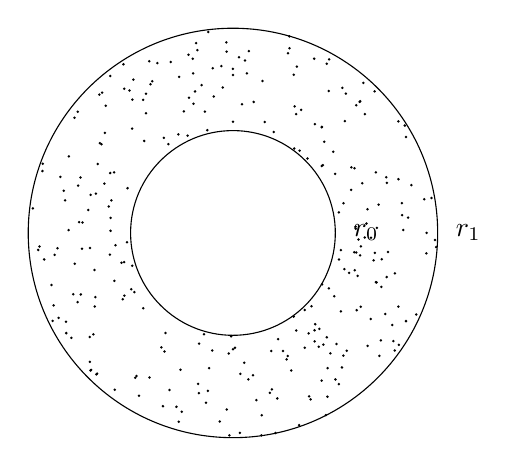
\begin{tikzpicture}[scale=1.3]
		% circles and line
		\draw (0,0) circle (1);
		\draw (0,0) circle (2);
		%\draw (0,0) -- (2,2);
	    %\node[thick] at (0,0) {\pgfuseplotmark{o}};
		%markings fro interval
		%\draw[thick] (0.8,0.8) -- (1.6,1.6);
		%\node[rotate=45, thick] at (0.8,0.8) {\pgfuseplotmark{|}};
		%\node[rotate=45, thick] at (1.6,1.6) {\pgfuseplotmark{|}};
		%\node[thick] at (1.2,1.2) {\pgfuseplotmark{*}};
		% labels
		%\node at (1.0,1.4) {$r_\tau$};
		\node at (1.3,0) {$r_0$};
		\node at (2.3,0) {$r_1$};
		% random points
		\foreach \x in {1,...,300}{
			\pgfmathsetmacro{\r}{sqrt(random(100,400)/100)}%
			\pgfmathsetmacro{\a}{random(0,360)}%
			\pgfmathsetmacro{\x}{\r*sin(\a)}
			\pgfmathsetmacro{\y}{\r*cos(\a)}
			\node[fill,circle,inner sep=0pt,minimum size=1pt] at (\x ,\y) {};
		}
	\end{tikzpicture}
	\end{subfigure}
	\begin{subfigure}[t]{0.5\textwidth}
		\centering
		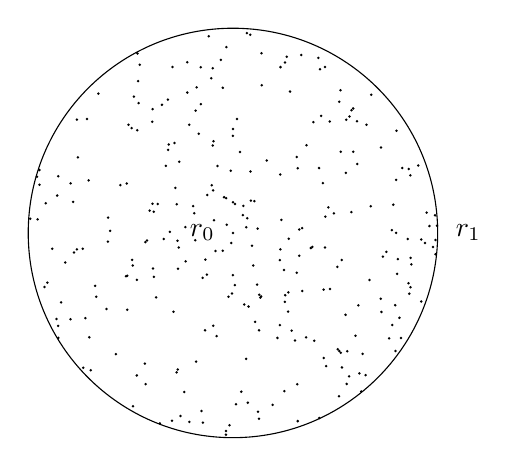
\begin{tikzpicture}[scale=1.3]
			% circles and line
			\draw (0,0) circle (2);
			%\draw (0,0) -- (2,2);
			%\node[thick] at (0,0) {\pgfuseplotmark{o}};
			%markings fro interval
			%\draw[thick] (0.0,0.0) -- (0.8,0.8);
			%\node[rotate=45, thick] at (0.8,0.8) {\pgfuseplotmark{|}};
			%\node[thick] at (0.3,0.3) {\pgfuseplotmark{*}};
			% labels
			%\node at (0.05,0.5) {$r_\tau$};
			\node at (-0.3,0) {$r_0$};
			\node at (2.3,0) {$r_1$};
			%\node at (1.0,0.6) {$r_\tau^*$};
			% random points
			\foreach \x in {1,...,300}{
				\pgfmathsetmacro{\r}{sqrt(random(0,400)/100)}%
				\pgfmathsetmacro{\a}{random(0,360)}%
				\pgfmathsetmacro{\x}{\r*sin(\a)}
				\pgfmathsetmacro{\y}{\r*cos(\a)}
				\node[fill,circle,inner sep=0pt,minimum size=1pt] at (\x ,\y) {};
			}
		\end{tikzpicture}
	\end{subfigure}
	\caption{The figure depicts the two topological cases for the support of the equilibrium measure - the droplet. On the left $r_0 > 0$ defining the annulus and on the right $r_0 =0$ defining the disk.}
\end{figure}

\begin{definicao} \label{Definition: Droplet}
	We call \textbf{Droplet} the support of $\mu_Q$, which in our case is the set of all complex values $z$ such that $r_0 \leq |z| \leq r_1$.
\end{definicao}

\section{Solving for the Free Energy}
\label{Section: Free eenrgy}

Remember the expression for the Gibbs-Boltzmann measure of Coulomb gases 
\begin{equation}
	\dd p_n ({\chi_n}) = \frac{1}{\pZ{n}{Q}} \ee^{-\beta n^2 \Hf(\chi_n)} \prod_{i = 1}^{n} \dd^d x_i.
\end{equation}
As discussed, this expression refers to a thermodynamic fluid of particles with positions ${\chi_n} = \mmany{x}{n}$ on a conductor $\Sigma$, in equilibrium at some inverse temperature $\beta$ an submitted to a confining potential $Q$ and a repulsive logarithmic term of interaction.  Because of the term $\beta n^2$, taking the asymptotic $n \rightarrow \infty$ means at the same time zero temperature and the thermodynamic limit. Physically, understanding the equilibrium positions would be equivalent to minimizing the \textit{Free Energy} $F = - (1/\beta) \ln \pZ{n}{Q}$. Let's describe the idea behind such minimization. This section \textit{is not rigorous}, its only purpose is to connect the idea of equilibrium problems with the asymptotics we will perform in \autoref{chapter: planarensembles} and elucidate where the expression for the free energy comes from. This argument, in more detail, can be found in \citeonline{Livan_2018}.

Lets first take the normalized counting measure, already introduced in \autoref{Section: RMT},
\begin{equation}
	\n(x) = \frac{1}{n} \sum_{i = 1}^{n} \delta(x - x_i).
\end{equation}
Note that using this function we write the unity as
\begin{equation}
	1 = \int \dd [\n(x)] \delta \left[ \n(x) - \frac{1}{n} \sum_{i=1}^{n} \delta(x - x_i) \right],
\end{equation}
we rewrite our partition function from \eqref{Equation: Equilibrium gas} as
\begin{equation}
	\pZ{n}{Q} = C_{n, \beta} \int \dd [\n(x)] \int_{\R^{dn}} \prod_{j=1}^{n} \dd x_j \ee^{-\beta n^2 \Hf(\chi_n)} \delta  \left[ \n(x) - \frac{1}{n} \sum_{i=1}^{n} \delta(x - x_i) \right].
\end{equation}
We do not want to deal with summations, in this context, integrals can be much easier to deal with. Then, we also want to convert the expression for the Hamiltonian. The confining term is easier, we write
\begin{equation}
	\frac{1}{n} \sum_{i=1}^{n} Q(x) = \frac{1}{n} n \int_{\R^d} n(x) Q(x) \dd x.
\end{equation}
For the interaction term, one must first note that
\begin{equation}
	\frac{1}{2n^2} \sum_{i \neq j} \ln |x_i - x_j| = \frac{1}{2n^2} \left[ \sum_{i,j} \ln |x_i - x_j| - \sum_i \Delta x_i \right]
\end{equation}
where we call $\Delta x_i$ is the cutoff distance and refers to the term $i = j$ in the discrete case and two neighboring charges approximating in the continuous case. This should ensure that the functional will still produce a finite result. Now we write
\begin{equation}
		\frac{1}{2n^2} \sum_{i \neq j} \ln |x_i - x_j| = \frac{1}{2n^2} n^2 \int \int_{\R^{2d}} \dd x \dd y \n(x) \n(y) \ln |x - y| - 	\frac{1}{2n^2} n \int_{\R^d} \dd x \n(x) \ln \Delta (x). 
\end{equation}
and then
\begin{align}
		\pZ{n}{Q}&  = C_{n, \beta} \int \dd [\n(x)] \ee^{-\beta n^2 \Hf(\n(x))} \int_{\R^{dn}} \prod_{j=1}^{n} \dd x_j \delta \left[ \n(x) - \frac{1}{n} \sum_{i=1}^{n} \delta(x - x_i) \right] \\
		& \revdeff  C_{n, \beta} \int \dd [\n(x)] \ee^{-\beta n^2 \Hf(\n(x))} I_n[\n(x)],
\end{align}
where
\begin{equation}
	\Hf(\n(x)) = \int_{\R^d} n(x) Q(x) \dd x + \frac{1}{2} \int \int_{\R^{2d}} \dd x \dd y \n(x) \n(y) \ln |x - y| - \frac{1}{2n} \int_{\R^d} \dd x \n(x) \ln \Delta (x). 
\end{equation}

Physically it is possible to think of  $I_n[\n(x)]$ as a count of how many microstates $\chi_n$ are compatible with the macrostate $\n(x)$. The logarithm of this quantity is proportional to the entropy of such system. Rewrite this function as
\begin{align}
	I_n[\n(x)] & = \int \dd [\n(x)] \int_{\R^{dn}} \prod_{j=1}^{n} \dd x_j \exp{ \left[\ii n \int \dd x \n(x) \hat{\n}(x) - \ii \int \dd x \hat{\n}(x) \sum_{i=1}^{n} \delta(x - x_i) \right]} \\
	& =  \int \dd [\n(x)]  \exp{\left[ \ii n \int_{\R^{dn}} \dd x \n(x) \hat{\n}(x) \right]} \left[ \int_{\R^d} \dd y \ee ^{\ii \int_{\R^d} \dd x \hat{\n}(x) \delta(x- x_i) } \right]^n \\
	& = \int \dd [\hat{\n}(x)] \ee^{n S[\hat{\n}(x) | \n(x)]},
	\label{Equation: logarithmic energyy - entropy}
\end{align}
where
\begin{equation}
	S[\hat{\n}(x) | \n(x)] = \ii \int_{\R^{dn}} \dd x \n(x) \hat{\n}(x) + \ln \int_{\R^d} \dd y \ee^{-\ii \hat{\n}(x)}.
\end{equation}

Notice here that \eqref{Equation: logarithmic energyy - entropy} is of a similar form from the one required by the Laplace asymptotic technique discussed in \autoref{chapter:asymptotics}. We estimate it, if $S$ has a maxima with strictly negative second derivative, by the evaluation at its maximum point. We find
\begin{align}
	0 & = \frac{\partial S}{\partial \hat{\n}(x)} = \ii \n(x) - \ii \frac{\ee^{-\ii \hat{\n}(x)}}{\int_{\R^d} \dd y \ee^{-\ii \hat{\n}(y)}} \\
	& \implies -\ii \hat{\n}(x) = -\ln(\n(x)) - \ln \int_{\R^{d}} \dd y \ee^{-\ii \hat{\n}(y)},
\end{align}
for the critical counting function. Then, substituting,
\begin{equation}
	I_n[\n(x)] \approx \exp{\left[ -n \int_{\R^{nd}} \dd x \n(x) \ln(\n(x)) \right]},
\end{equation}
which has the form of the Shannon entropy of the density $\n(x)$. There is a classical argument that states that $\Delta(x) \approx c / (n \n(x))$, i.e., the higher the density of particles around a point $x$, the smaller the average distance between them. Thus, 
\begin{align}
	\int_{\R^d} \dd x \n(x) \ln \Delta (x) & \approx \int_{\R^d} \dd x \n(x) \ln\left( \frac{c}{n \n(x)}\right)  \\
	& = \int_{\R^d} \dd x \n(x) \left(\ln c - \ln n + \ln \n(x) \right) \\
	& = \int_{\R^d} \dd x \n(x) \ln c  - \int_{\R^d} \dd x \n(x) \ln n + \int_{\R^d} \dd x \n(x) \ln \n(x).
\end{align}
Return now to the partition function and use the relations found to write
\begin{align}
		\pZ{n}{Q} & \approx C_{n, \beta} \int \dd [\n(x)] \exp{\left[-\beta n^2 \Hf(\n(x))\right]} \exp{\left[ -n \int_{\R^{nd}} \dd x \n(x) \ln(\n(x)) \right]}, \\
		&  \approx C_{n, \beta} \int \dd [\n(x)] \exp{\left[-\beta n^2 \mathfrak{F}_0[\n(x)] + \frac{\beta n}{2} \mathfrak{F}_1[\n(x)] + \frac{\beta}{2} n \ln(n) - \frac{\beta}{2} n \ln (c) \right]} \exp{\left[ -n \mathfrak{F}_1[\n(x)] \right]}, \\
		& \approx C_{n, \beta} \int \dd [\n(x)] \exp{\left[-\beta n^2 \mathfrak{F}_0[\n(x)] + \frac{\beta}{2} n \ln(n) + n \left(\frac{\beta}{2} - 1\right) \mathfrak{F}_1[\n(x)] - \frac{\beta}{2} n \ln (c) \right]},
\end{align}
where
\begin{align}
	& \mathfrak{F}_0[\n(x)] \deff  \int_{\R^d} \n(x) Q(x) \dd x + \frac{1}{2} \int \int_{\R^{2d}} \dd x \dd y \n(x) \n(y) \ln |x - y|, \\
	& \mathfrak{F}_1[\n(x)] \deff  \int_{\R^d} \dd x \n(x) \ln \n(x).
\end{align}
Note that, now, one again perform a saddle point estimation for the asymptotic in a critical point $\n^*(x)$ to get
\begin{equation}
	\pZ{n}{Q} \approx \exp{\left[-\beta n^2 \mathfrak{F}_0[\n^*(x)] + \frac{\beta}{2} n \ln(n) + n \left(\frac{\beta}{2} - 1\right) \mathfrak{F}_1[\n^*(x)] - \frac{\beta}{2} n \ln (c) \right]}
\end{equation}
and finally for the Free Energy
\begin{equation}
	\ln(\pZ{n}{Q}) = -\beta n^2 \mathfrak{F}_0[\n^*(x)] + \frac{\beta}{2} n \ln(n) + n \left(\frac{\beta}{2} - 1\right) \mathfrak{F}_1[\n^*(x)] - \frac{\beta}{2} n \ln (c) + \Boh(n).
\end{equation}
Obtaining a expression for the Free Energy when $\beta = 2$, rigorously, is the main goal for \autoref{chapter: planarensembles}. 